\chapter{Systemarkitektur - Hardware}

\begin{figure}[h!]
	\centering
	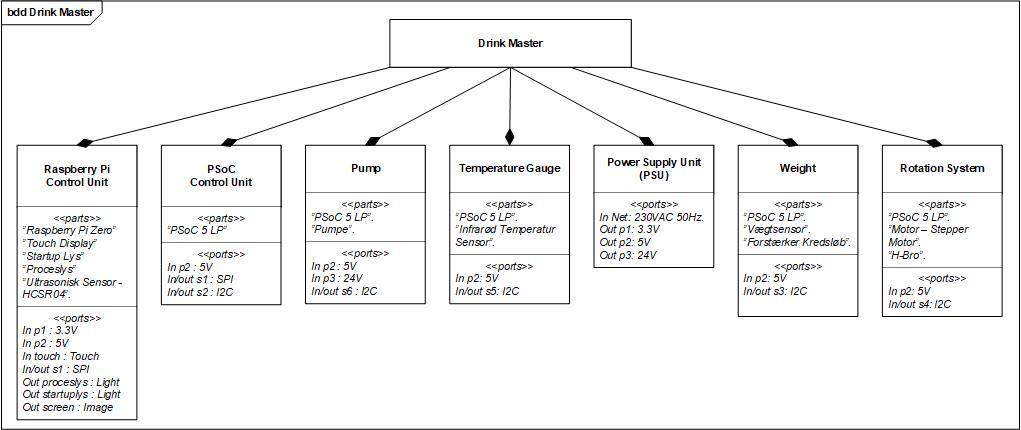
\includegraphics[width=1.2\textwidth, angle =270]{Images/BDD_System_JPEG.jpg}
	\caption{bdd for Drink master}
	\label{fig:bdd}
\end{figure}
\FloatBarrier

\begin{table}[!h] 
	\centering 
	\caption{Blokbeskrivelse for figur \ref{fig:bdd} bdd Drink master}
	\begin{tabular}{|p{3cm}|p{7cm}|p{3cm}|}
		\hline
\textbf{Bloknavn} & \textbf{Funktionsbeskrivelse}  &  \textbf{Kommentar}  \\ \hline
Raspberry Pi control unit    & Raspberry Pi SPI Master-enhed. Er forbundet med et Touch Display, som er brugerens tilgang til systemet. Der er også forbundet med en ultralydssensor som tænder lys i system når en bruger er tæt på. Kommunikerer med PSoC I2C Master-enhed. &  \\ \hline
PSoC control unit & I2C Master-enhed, som kommunikerer direkte med alle andre enheder. Danner et kommunikationsled mellem alle I2C PSoC Slaver og RPi SPI Master.    &  \\ \hline
Pump              & En pumpe der pumper en prædefineret mængde af væske fra en flaske ned i et indsat krus, som skal mixes i den valgte drink.                       &  \\ \hline
Temperature Gauge & En Infrarød Temperatur Sensor detekterer temperaturen på flasker.                                                                                &  \\ \hline
PSU               & En strømforsyning som leverer de forskellige spændinger som systemet har brug for.                                                                               &  \\  \hline
Weight            & Et vægtsystem til at registrere indsat krus, før en drik kan laves, og om væske er påfyldt kruset.                                                                      &  \\ \hline
Rotation System   & En motor styrer et hjul med flasker. En flaske, som skal bruges til en valgt drink bliver positioneret ovenover et indsat krus.                  &  \\ \hline

		\hline 
	\end{tabular}
	\label{tab:blokbeskrivelse}
\end{table}
\FloatBarrier

\begin{figure}[h!]
	\centering
	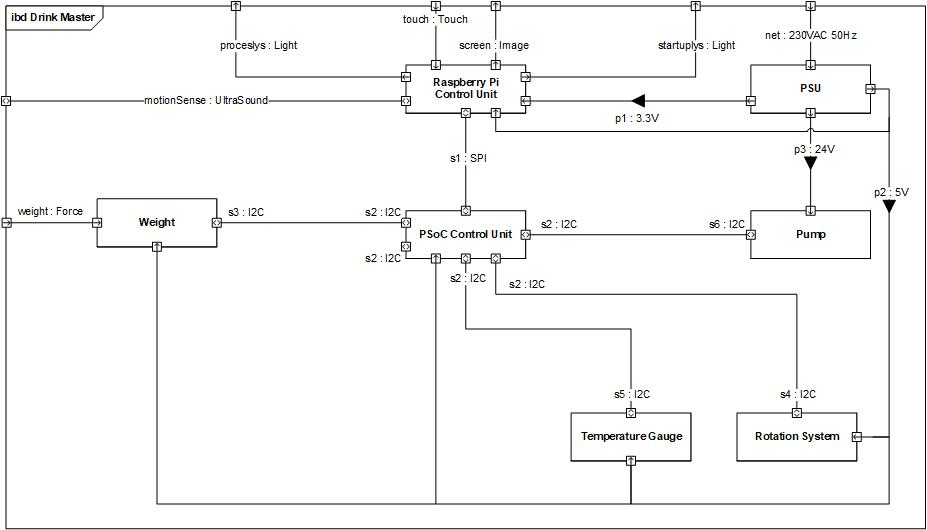
\includegraphics[width=1\textwidth]{Images/IBD_System_JPEG.jpg}
	\caption{ibd for Drink master}
	\label{fig:ibd}
\end{figure}
\FloatBarrier

\begin{table}[!h] 
	\centering 
	\caption{Signalbeskrivelse for figur \ref{fig:ibd} ibd Drink master}
	\begin{tabular}{|p{3cm}|p{7cm}|p{3cm}|}
		\hline
\textbf{Signal} & \textbf{Funktionsbeskrivelse}  &  \textbf{Kommentar}  \\ \hline
Raspberry Pi control unit   & &  \\ \hline
PSoC control unit    & &  \\ \hline
Pump              & &  \\ \hline
Temperature Gauge & &  \\ \hline
PSU               & &  \\ \hline 
Weight            & &  \\ \hline
Rotation System   & &  \\ \hline

	\end{tabular}
	\label{tab:signalbeskrivelse}
\end{table}
\FloatBarrier